\section{Methodology}

\subsection{Problem Formulation}

Let $\mathbf{X} \in \mathbb{R}^{T \times N}$ denote a multivariate time series of $T$ observations over $N$ variables. We assume the underlying data-generating process is a nonstationary Structural Vector Autoregressive (SVAR) model defined by a discrete latent regime variable $S_t \in \{1, \dots, M\}$:
\begin{equation}
    \mathbf{X}_t = \sum_{\tau=1}^{L} \mathbf{A}^{(\tau, S_t)} \mathbf{X}_{t-\tau} + \boldsymbol{\varepsilon}_t, \quad \boldsymbol{\varepsilon}_t \sim \mathcal{N}(\mathbf{0}, \boldsymbol{\Sigma}^{(S_t)})
\end{equation}
where $L$ is the maximum temporal lag, $\mathbf{A}^{(\tau, S_t)} \in \mathbb{R}^{N \times N}$ is the regime-dependent transition matrix at lag $\tau$ during hidden state $S_t$, and $\boldsymbol{\varepsilon}_t$ is zero-mean, regime-specific Gaussian noise. The target is to infer the global summary causal graph $\mathcal{G} = (\mathcal{V}, \mathcal{E})$, where a directed edge $(i \rightarrow j) \in \mathcal{E}$ denotes that variable $i$ Granger-causes variable $j$ under at least one regime. REIGN operates through four cascading stages to recover $\mathcal{G}$ from purely observational data, as illustrated in Fig. \ref{fig:pipeline}.

\begin{figure}[htbp]
\centerline{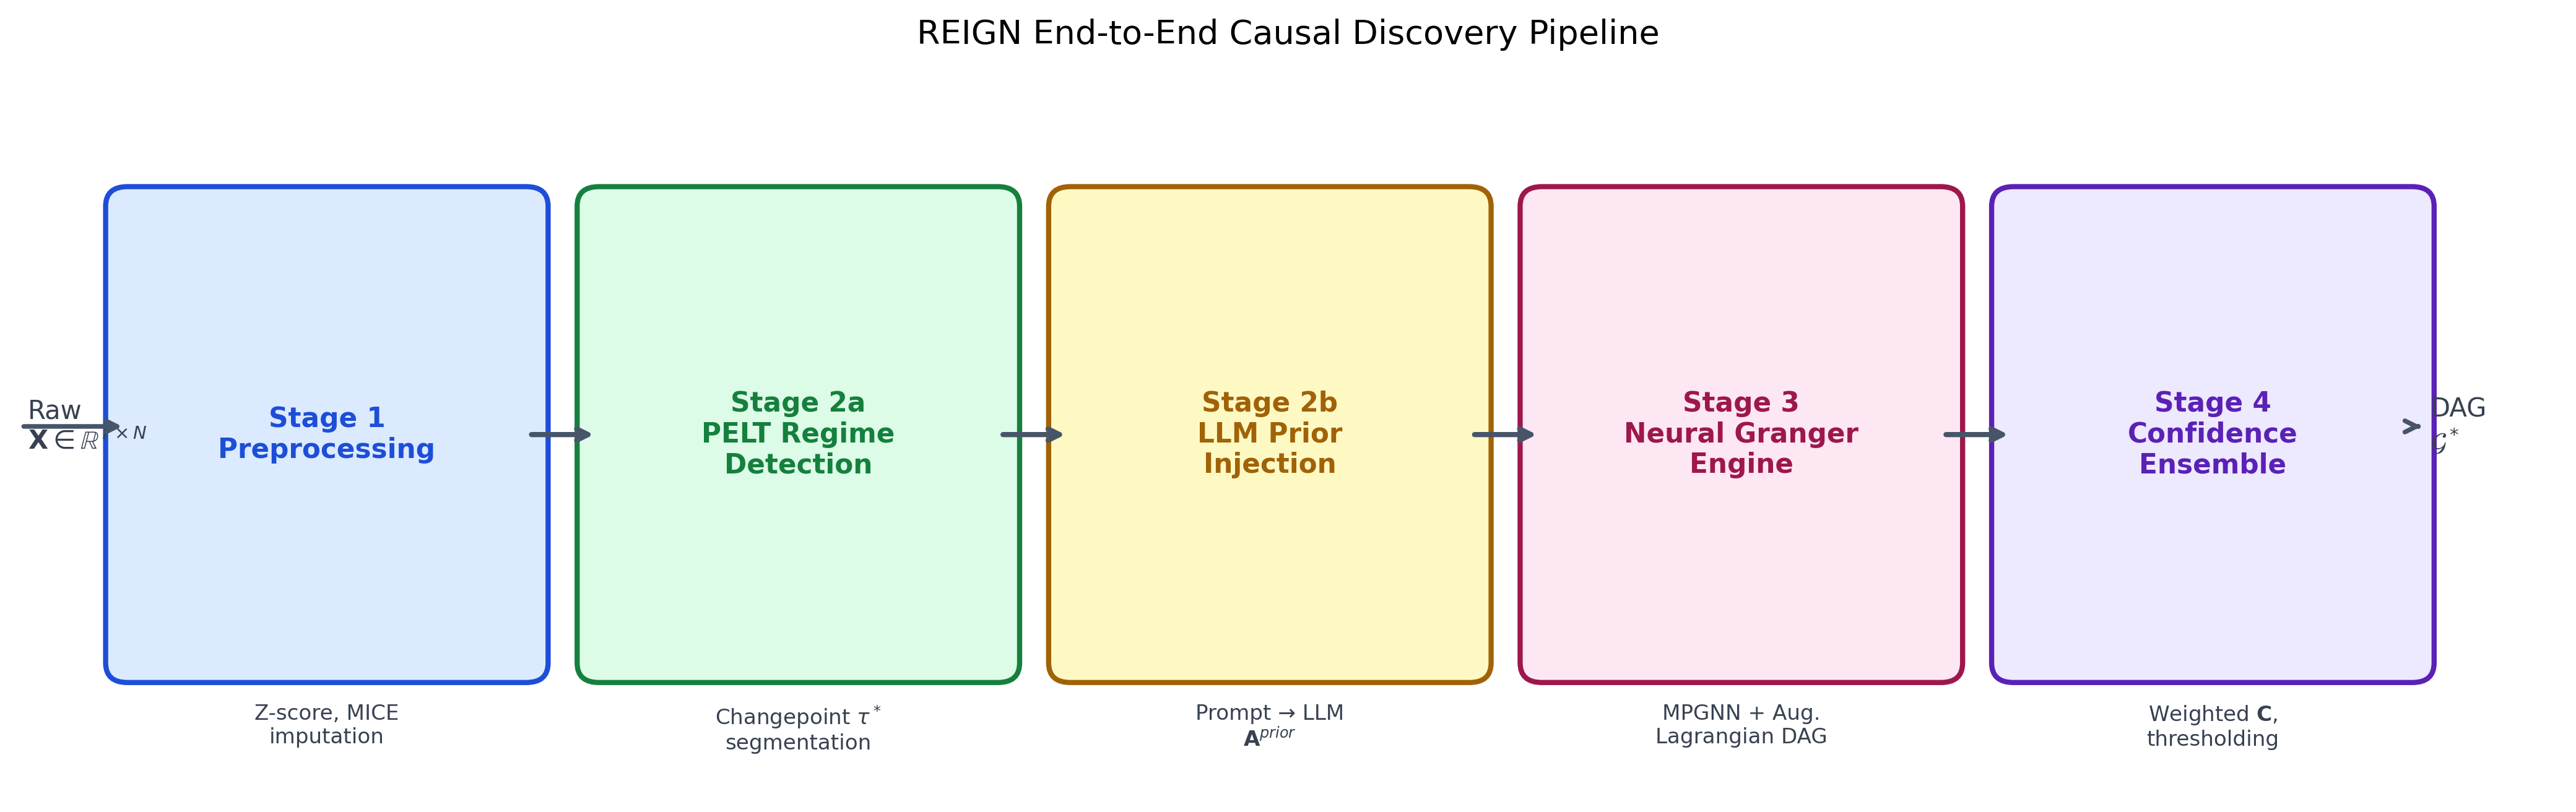
\includegraphics[width=\columnwidth]{figures/5_reign_pipeline.png}}
\caption{The REIGN end-to-end causal discovery pipeline. Raw multivariate time series $\mathbf{X}$ passes sequentially through robust preprocessing (Stage 1), PELT-based regime segmentation (Stage 2a), LLM prior injection (Stage 2b), per-regime MPGNN training (Stage 3), and confidence-weighted ensemble aggregation (Stage 4) to produce the final DAG $\mathcal{G}^*$.}
\label{fig:pipeline}
\end{figure}

\subsection{Stage 1: Robust Preprocessing}

Financial and physiological time series commonly contain missing data segments and extreme measurement anomalies. We apply the following preprocessing pipeline:

\begin{enumerate}
    \item \textbf{Z-score normalization:} Each channel $X^{(n)}$ is standardized using robust estimates of location and scale computed from non-missing entries.
    \item \textbf{Outlier flagging:} Entries where $|X_t^{(n)} - \mu_n| > 3\sigma_n$ are flagged and treated as missing.
    \item \textbf{MICE Imputation:} Missing entries are imputed using Multiple Imputation by Chained Equations (MICE), which iteratively fits a sequence of conditional models $p(X^{(n)} | \mathbf{X}^{(-n)})$ to preserve the inter-channel covariance structure critical to Granger causality detection.
\end{enumerate}

\subsection{Stage 2a: Statistical Regime Detection via PELT}

We model the regime shifts as a sequence of abrupt changepoints partitioning $[1, T]$ into $K+1$ contiguous segments. The Pruned Exact Linear Time (PELT) algorithm \cite{Killick2012} efficiently identifies the optimal set of changepoints $\mathcal{T}^* = \{\tau_1^*, \dots, \tau_K^*\}$ by minimizing the penalized total cost:
\begin{equation}
    \mathcal{T}^* = \underset{K, \mathcal{T}}{\arg\min} \left\{ \sum_{k=0}^{K} \mathcal{C}\left(\mathbf{X}_{(\tau_k, \tau_{k+1}]}\right) + \beta (K+1) \right\}
\end{equation}
where $\mathcal{C}(\cdot)$ is a within-segment cost (we use the negative log-likelihood of a Gaussian fit to rolling covariance), and $\beta > 0$ is the penalty controlling the trade-off between segment count and goodness-of-fit. PELT operates with worst-case $\mathcal{O}(T)$ complexity by exploiting a pruning inequality discarding non-optimal changepoint candidates. Segments shorter than a minimum length $T_{min}$ are merged into adjacent partitions to ensure sufficient samples for stable neural training. The PELT segmentation and the resulting cost signal are visualised in Fig. \ref{fig:pelt}.

\begin{figure}[htbp]
\centerline{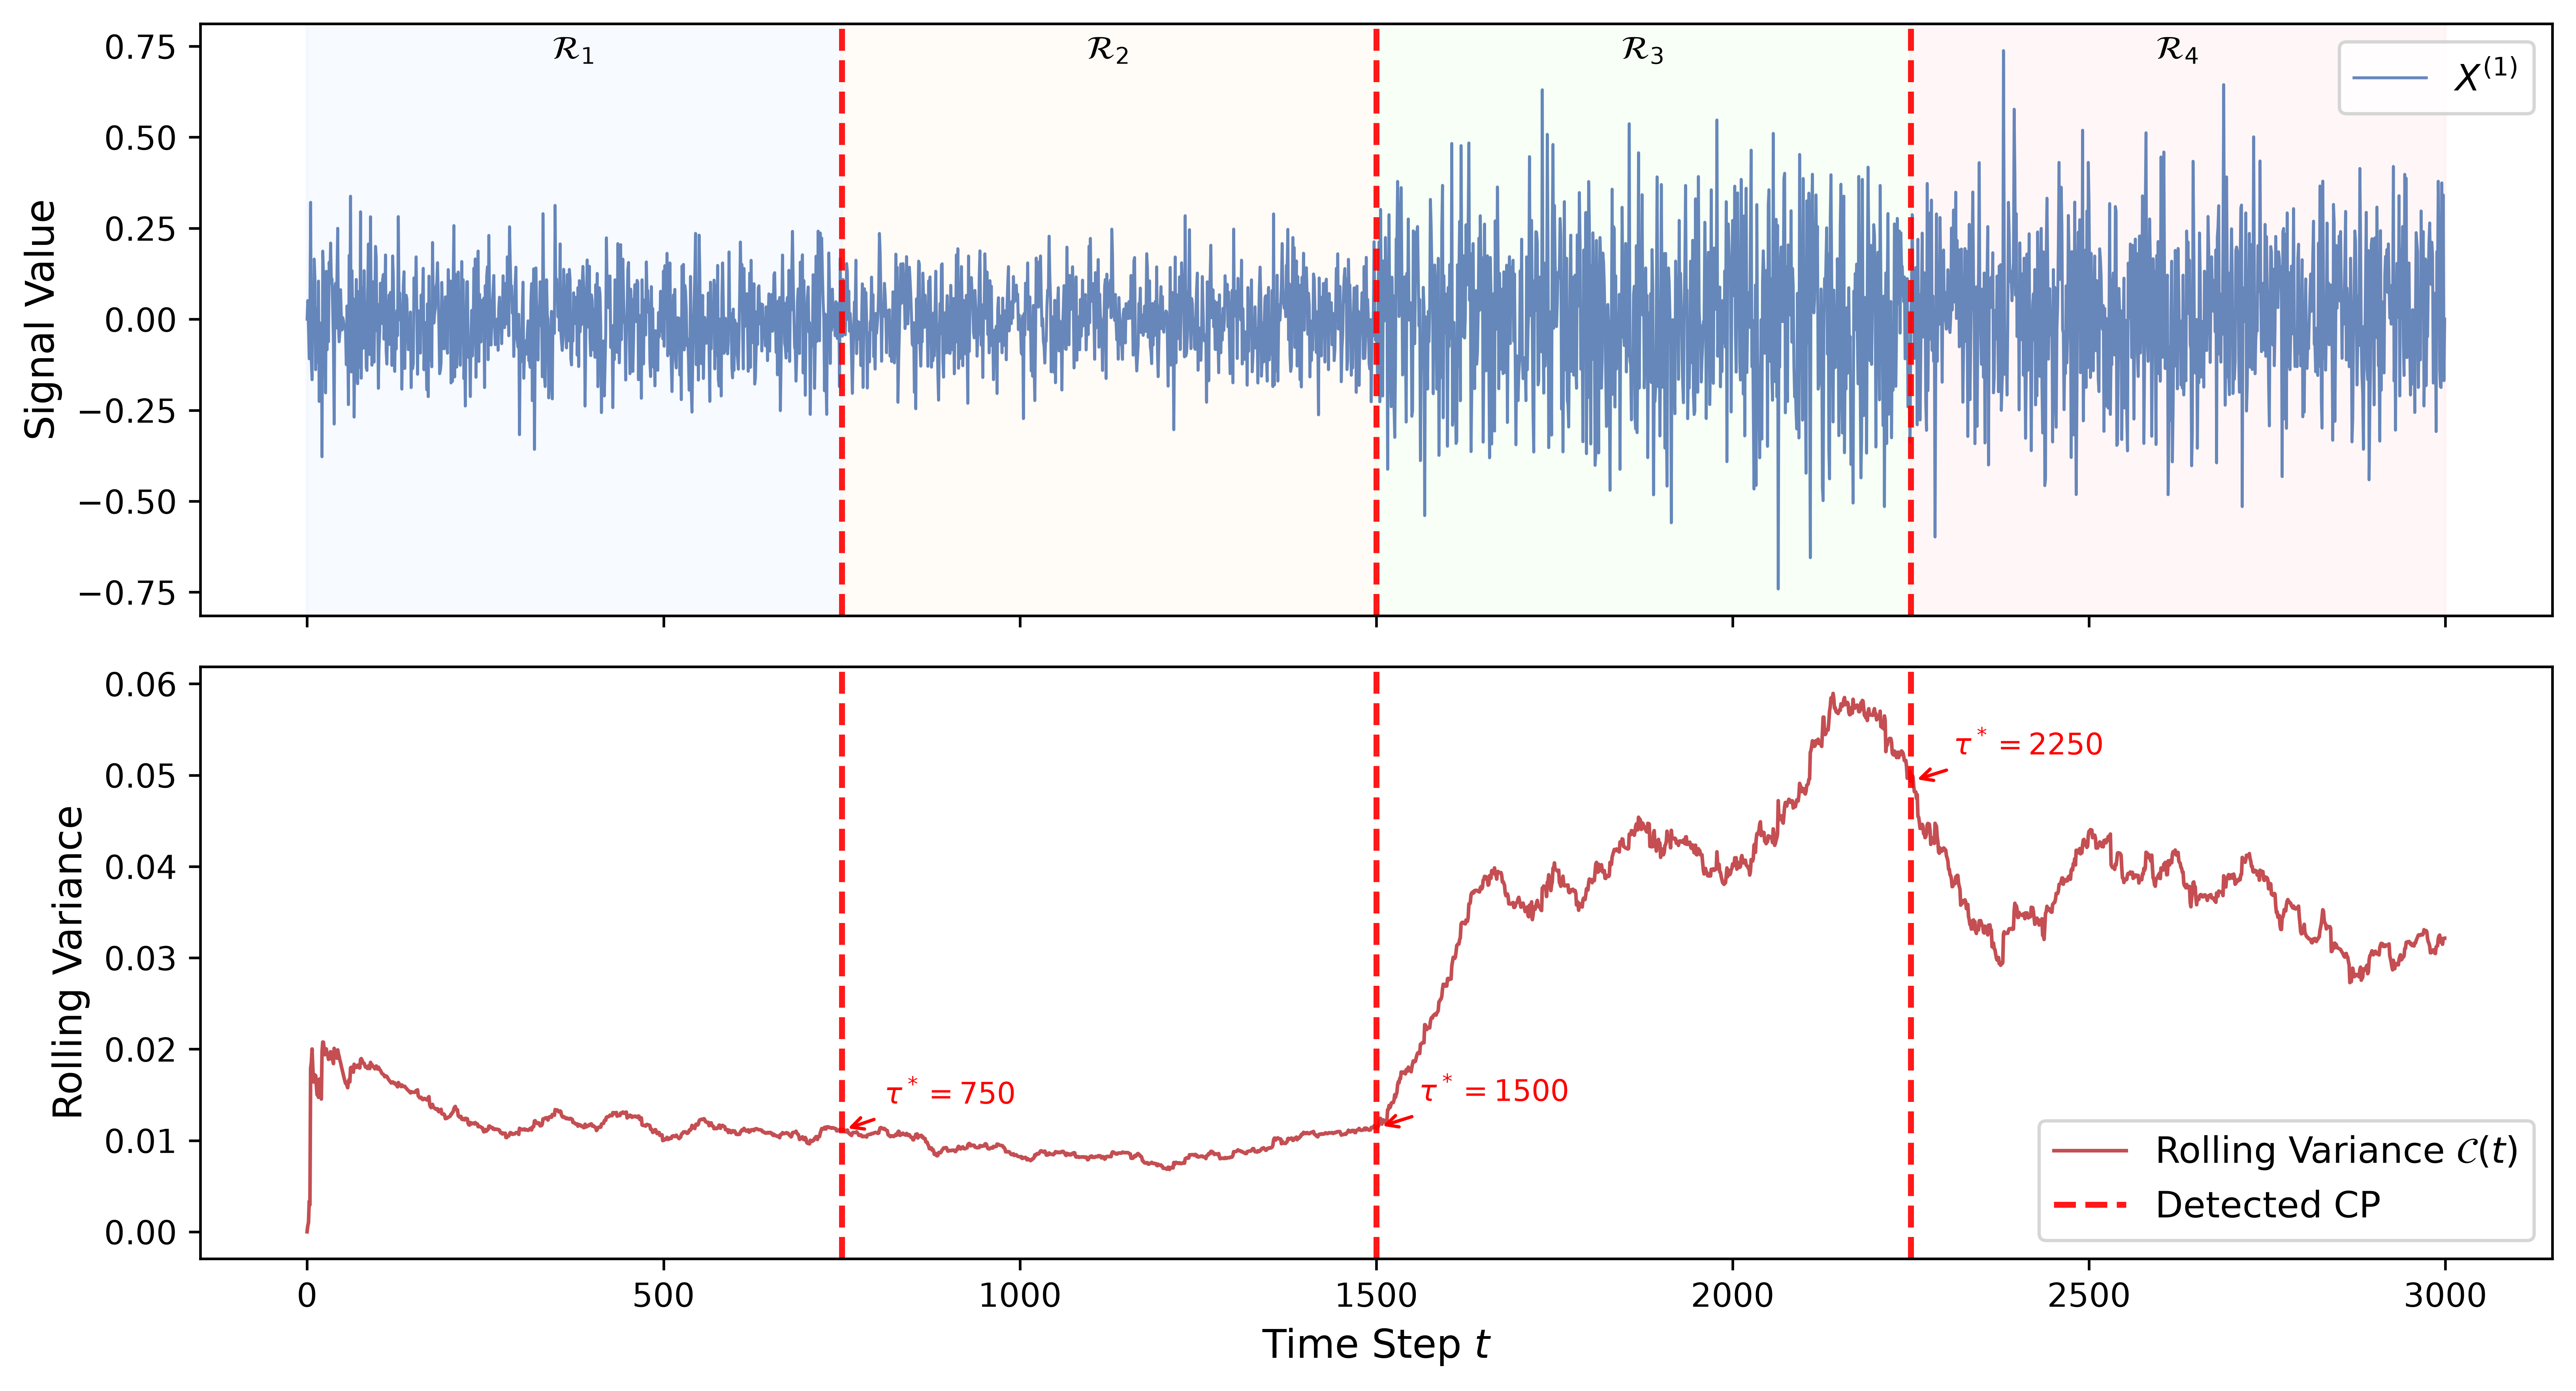
\includegraphics[width=\columnwidth]{figures/6_pelt_segmentation.png}}
\caption{PELT changepoint detection applied to the synthetic VAR dataset. (Top) The raw signal $X^{(1)}$ with detected changepoints (red dashed lines) and shaded regime windows $\mathcal{R}_1$–$\mathcal{R}_4$. (Bottom) The rolling variance cost signal $\mathcal{C}(t)$ used by PELT, with sharp peaks at regime transition boundaries clearly indicating distributional shifts.}
\label{fig:pelt}
\end{figure}

\subsection{Stage 2b: Zero-Shot LLM Prior Injection}

Unconstrained neural causal discovery over an $N$-node graph faces a search space of $2^{N(N-1)}$ possible DAGs, which is computationally intractable for $N > 20$ without strong inductive biases. REIGN generates these inductive biases from a zero-shot Large Language Model query.

Given a natural language description of each variable and a domain context, we construct a structured prompt $\mathcal{P}$ and query an LLM (e.g., Anthropic Claude). The model returns a confidence score $p_{ij} \in [0, 1]$ for each ordered pair $(i, j)$, representing the LLM's belief in the causal link $i \rightarrow j$. These scores assemble into a prior matrix $\mathbf{A}^{prior} \in [0,1]^{N \times N}$.

To guarantee topological consistency, $\mathbf{A}^{prior}$ is post-processed via a confidence-weighted Kahn's algorithm to compute the implied topological ordering. Any edges violating this order are masked, ensuring $\mathbf{A}^{prior}$ is already acyclic before entering Stage 3.

\subsection{Stage 3: Coarse-to-Fine Neural Granger Engine}

For each regime $\mathcal{R}_k$, we extract the corresponding slice $\mathbf{X}^{(k)} \in \mathbb{R}^{T_k \times N}$ and deploy an adapted Message-Passing Graph Neural Network (MPGNN) \cite{Cheng2024}. Unlike prior works that employ a LASSO bottleneck as a coarse-discovery prefilter, REIGN initializes $\mathbf{W}^{(k)}$ as a fully connected dense topology, preventing premature truncation of weak but genuine causal signals.

The GNN takes a historical window as input and propagates messages along the current graph estimate:
\begin{equation}
    \mathbf{h}_i^{(l+1)} = \phi\left(\mathbf{h}_i^{(l)},\; \bigoplus_{j} W^{(k)}_{ji} \cdot \psi\left(\mathbf{h}_j^{(l)}\right)\right)
\end{equation}
where $\mathbf{h}_i^{(l)}$ is the hidden state of node $i$ at GNN layer $l$, $\phi$ and $\psi$ are learnable MLP transformations, and $\bigoplus$ denotes weighted sum aggregation.

The training objective combines temporal prediction, LLM prior regularization, acyclicity, and sparsity:
\begin{equation}
    \mathcal{L}(\mathbf{W}^{(k)}) = \frac{1}{T_k}\sum_t\|\hat{\mathbf{X}}_t - \mathbf{X}_t\|_2^2 + \lambda \|\mathbf{W}^{(k)} - \mathbf{A}^{prior}\|_F^2 + \gamma \|\mathbf{W}^{(k)}\|_1
\end{equation}
subject to the continuous DAG constraint $h(\mathbf{W}^{(k)}) = \text{tr}(e^{\mathbf{W}^{(k)} \circ \mathbf{W}^{(k)}}) - N = 0$.

This constraint is handled via an Augmented Lagrangian scheme with dual variable $\mu^{(k)}$ and penalty $\rho^{(k)}$:
\begin{equation}
    \mathcal{L}_{AL} = \mathcal{L}(\mathbf{W}^{(k)}) + \mu^{(k)} h(\mathbf{W}^{(k)}) + \frac{\rho^{(k)}}{2}\left|h(\mathbf{W}^{(k)})\right|^2
\end{equation}
We optimize via Adam and update $\mu^{(k)} \leftarrow \mu^{(k)} + \rho^{(k)} h(\mathbf{W}^{(k)})$ and $\rho^{(k)} \leftarrow \eta \rho^{(k)}$ at each outer iteration until $h(\mathbf{W}^{(k)}) < \epsilon_{tol}$.

\subsection{Stage 4: Confidence-Weighted Ensemble}

Each regime $\mathcal{R}_k$ yields a continuous causal weight matrix $\mathbf{W}^{(k)}$. To synthesize a global summary causal graph, REIGN performs temporal-duration-weighted aggregation:
\begin{equation}
    \mathbf{C} = \sum_{k=1}^{K} \omega_k \cdot \text{sigmoid}\left(|\mathbf{W}^{(k)}|\right), \quad \omega_k = \frac{T_k}{\sum_{j=1}^K T_j}
\end{equation}
\begin{revenv}
The resulting confidence matrix $\mathbf{C} \in (0,1)^{N \times N}$ serves as the continuous causal estimate. The binary summary graph $\mathcal{G}^*$ is recovered by applying a threshold $\tau$:
\begin{equation}
    \mathcal{G}^*_{ij} = \mathbf{1}[\mathbf{C}_{ij} > \tau]
\end{equation}
In practical deployments where the ground-truth graph $\mathbf{G}_{true}$ is unavailable, $\tau$ cannot be selected by maximizing the F1 score against the ground truth. Instead, $\tau$ should be determined via a fixed domain-specific threshold (e.g., $\tau = 0.5$) or calibrated on a structurally similar validation dataset where structural metrics are observable. In our experiments, we explore both fixed thresholds and calibration metrics to reflect realistic operational settings.

\subsection{Theoretical Consistency of the Ensemble}

The confidence-weighted aggregation mechanism is theoretically justified under standard consistency assumptions. 

\textbf{Proposition 1.} \textit{Assume that the PELT algorithm correctly identifies the true regime changepoints $\mathcal{T}^*$ as $T \to \infty$. Let the MPGNN estimator $\hat{\mathbf{W}}^{(k)}$ for each regime $\mathcal{R}_k$ be asymptotically consistent, such that $\hat{\mathbf{W}}^{(k)} \xrightarrow{p} \mathbf{W}^{(k)}_{true}$ as $T_k \to \infty$. Then, the weighted confidence matrix $\mathbf{C}$ converges in probability to the true temporally-weighted structural expectation:}
\begin{equation}
    \mathbf{C} \xrightarrow{p} \sum_{k=1}^{K} \omega^*_k \cdot \text{sigmoid}\left(|\mathbf{W}^{(k)}_{true}|\right)
\end{equation}
\textit{where $\omega^*_k$ is the true underlying temporal proportion of regime $k$.}

This proposition ensures that in the limit of sufficient data within each regime and accurate changepoint detection, the aggregated confidence matrix faithfully recovers the global causal structure without asymptotically vanishing signals from transient regimes.
\end{revenv}
A final depth-first cycle elimination pass ensures $\mathcal{G}^*$ is a valid DAG.

\subsection{Hyperparameter Summary}

\begin{table}[htbp]
\centering
\caption{REIGN Hyperparameter Configuration}
\label{tab:hyperparams}
\begin{tabular}{llp{4.2cm}}
\toprule
\textbf{Parameter} & \textbf{Value} & \textbf{Description} \\
\midrule
$L$ (lag)         & 5       & Maximum temporal lag \\
$\beta$ (PELT)    & 100     & Changepoint penalty \\
$T_{min}$         & 200     & Minimum regime length \\
$\lambda$ (prior) & \rev{0.1}     & LLM prior weight \\
$\gamma$ (sparsity) & 0.01 & $L_1$ regularization \\
Epochs            & 200     & GNN training steps per regime \\
Learning rate     & 1e-2    & Adam optimizer \\
$\eta$ (AL)       & 10.0    & Augmented Lagrangian growth \\
$\epsilon_{tol}$  & 1e-8    & DAG constraint tolerance \\
\bottomrule
\end{tabular}
\end{table}
